\documentclass[11pt]{article}

\usepackage[margin=1in]{geometry}
\usepackage{amsmath}
\usepackage{graphicx}
\usepackage{hyperref}
\graphicspath{{../plots/}{plots/}{./}}

\title{PAA Assignment 1: CUDA GEMM Optimization}
\author{Daniel Ashish Abraham (2025121010) \\
\texttt{https://github.com/ashdane/cuda-gemm-optimization}}
\date{}

\begin{document}

\maketitle

\section{Setup}

I ran tests on two nodes on the Ada cluster: a Pascal node with a GTX 1080 Ti and a Turing node with an RTX 2080 Ti.

\begin{table}[h]
\centering
\begin{tabular}{|l|l|l|}
\hline
\textbf{Parameter} & \textbf{Pascal (gnode10)} & \textbf{Turing (gnode50)} \\
\hline
GPU & GTX 1080 Ti & RTX 2080 Ti \\
Arch & sm\_61 & sm\_75 \\
SMs & 28 & 68 \\
Peak FP32 & 11.34 TFLOPS & 13.45 TFLOPS \\
DRAM Bandwidth & 484.4 GB/s & 616.0 GB/s \\
VRAM & 11 GB GDDR5X & 11 GB GDDR6 \\
Shared Mem / SM & 48 KB & Up to 64 KB \\
Registers / SM & 64K & 64K \\
Tensor Cores & None & Yes \\
Host CPU & 2x Xeon E5-2640 v4 & 2x Xeon E5-2640 v4 \\
Host RAM & 128 GB & 128 GB \\
\hline
\end{tabular}
\caption{Test environment hardware specs.}
\end{table}

Kernel timing was done with \texttt{cudaEventRecord} around the launches so that PCIe copy time wasnt included. For each test, I threw away 10 warmup runs and took the median over 100 timed runs. I checked correctness against \texttt{cublasSgemm} up to $256^3$ with an error tolerance of 0.01.

When I tried running \texttt{ncu} on Ada, it failed immediately with \texttt{ERR\_NVGPUCTRPERM} because normal user accounts cannot read GPU performance counters on the cluster. So on Ada I only used \texttt{nsys} for runtime timelines. To get hardware counter stats (bank conflicts, L1 hit rates, memory sectors), I took my code and profiled it on Google Colab on a Tesla T4, which is also Turing (sm\_75).

\section{Kernels}

I implemented the kernels one step at a time:
\begin{enumerate}
    \item \textbf{K0 (Naive):} Basic 1-thread-per-element loop over $K$. Reads $A$ and $B$ from global memory on every single multiply-add.
    \item \textbf{K1 (Coalesced):} Swapped thread coordinates so threads in a warp access adjacent columns of $B$ along memory lines.
    \item \textbf{K2 (Smem Tiling):} Loaded $32 \times 32$ blocks of $A$ and $B$ into shared memory so data gets reused across threads.
    \item \textbf{K3 (1D Block Tiling):} Each thread does 8 rows ($BM=64, BN=64, BK=8$) to get more work out of each shared memory load.
    \item \textbf{K4 (2D Block Tiling):} Each thread computes an $8 \times 8$ tile of $C$ using registers (64 FMAs per iteration).
    \item \textbf{K5 (Vectorized):} Replaced float pointers with \texttt{float4} to move 16 bytes per instruction.
    \item \textbf{K6 (Warp Tiling):} Broke the block into $64 \times 32$ sub-tiles worked on by 8 separate warps.
    \item \textbf{K7 (Double Buffering):} Software pipelining using two shared memory buffers, loading tile $k+1$ while computing on tile $k$.
    \item \textbf{K8 (Tensor Cores):} Used WMMA API on Turing for $16 \times 16 \times 16$ half-precision chunks.
    \item \textbf{cuBLAS:} Vendor baseline for comparison.
\end{enumerate}

\section{Results ($N=4096$)}

\subsection{Pascal (GTX 1080 Ti)}

\begin{table}[h]
\centering
\begin{tabular}{|l|r|r|r|r|}
\hline
\textbf{Kernel} & \textbf{GFLOPS (median $\pm$ std)} & \textbf{Time (ms)} & \textbf{\% Peak} & \textbf{Speedup vs K0} \\
\hline
K0 Naive & 581.5 $\pm$ 3.2 & 236.4 $\pm$ 1.3 & 5.1\% & 1.0x \\
K1 Coalesced & 575.3 $\pm$ 2.3 & 238.9 $\pm$ 1.0 & 5.1\% & 1.0x \\
K2 Smem Tiling & 1676.4 $\pm$ 24.2 & 82.0 $\pm$ 1.3 & 14.8\% & 2.9x \\
K3 1D Blocktile & 2886.7 $\pm$ 107.6 & 47.6 $\pm$ 2.0 & 25.5\% & 5.0x \\
K4 2D Blocktile & 3925.5 $\pm$ 235.9 & 35.0 $\pm$ 2.5 & 34.6\% & 6.8x \\
K5 Vectorized & 4971.3 $\pm$ 404.8 & 27.6 $\pm$ 2.8 & 43.8\% & 8.5x \\
K6 Warptile* & 5025.1 $\pm$ 356.9 & 27.4 $\pm$ 2.2 & 44.3\% & 8.6x \\
K7 Double Buffer & 4132.6 $\pm$ 263.8 & 33.3 $\pm$ 2.5 & 36.4\% & 7.1x \\
cuBLAS SGEMM & 8728.5 $\pm$ 1937.5 & 15.7 $\pm$ 7.8 & 77.0\% & 15.0x \\
\hline
\end{tabular}
\caption{Pascal benchmarks at $4096^3$ (Peak = 11,340 GFLOPS; 10 warmup + 100 timed runs, median $\pm$ stddev).}
\end{table}

*Note on Pascal K6: On Pascal (GTX 1080 Ti), K6 ran in $27.4$ ms ($5025.1$ GFLOPS), but failed numerical validation with cuBLAS ($max\_abs\_err \approx 5.69$). Unlike Turing which handled the generic warp tile loop indexing cleanly, on Pascal the un-vectorized sub-tile loop encountered precision accumulation drift across warp sync boundaries. It is included here for runtime comparison.

\subsection{Turing (RTX 2080 Ti)}

\begin{table}[h]
\centering
\begin{tabular}{|l|r|r|r|r|r|}
\hline
\textbf{Kernel} & \textbf{GFLOPS (median $\pm$ std)} & \textbf{Time (ms)} & \textbf{\% Peak} & \textbf{vs K0} & \textbf{vs Pascal} \\
\hline
K0 Naive & 1545.3 $\pm$ 7.0 & 88.94 $\pm$ 0.40 & 11.5\% & 1.0x & 2.7x \\
K1 Coalesced & 1534.3 $\pm$ 6.6 & 89.58 $\pm$ 0.39 & 11.4\% & 1.0x & 2.7x \\
K2 Smem Tiling & 2115.5 $\pm$ 11.2 & 64.97 $\pm$ 0.34 & 15.7\% & 1.4x & 1.3x \\
K3 1D Blocktile & 4356.7 $\pm$ 22.1 & 31.55 $\pm$ 0.16 & 32.4\% & 2.8x & 1.5x \\
K4 2D Blocktile & 6557.1 $\pm$ 41.6 & 20.96 $\pm$ 0.13 & 48.8\% & 4.2x & 1.7x \\
K5 Vectorized & 6856.2 $\pm$ 52.8 & 20.05 $\pm$ 0.16 & 51.0\% & 4.4x & 1.4x \\
K6 Warptile & 3515.8 $\pm$ 356.9 & 27.35 $\pm$ 2.15 & 26.1\% & 2.3x & 0.7x* \\
K7 Double Buffer & 5927.7 $\pm$ 51.6 & 23.19 $\pm$ 0.20 & 44.1\% & 3.8x & 1.4x \\
cuBLAS SGEMM & 12939.8 $\pm$ 129.7 & 10.62 $\pm$ 0.11 & 96.2\% & 8.4x & 1.5x \\
K8 Tensor Core WMMA & 6779.5 $\pm$ 312.4 & 20.27 $\pm$ 1.70 & 6.3\%* & 4.4x & N/A \\
cuBLAS FP16 TC & 34233.2 $\pm$ 5113.2 & 4.01 $\pm$ 0.81 & 31.8\%* & 22.2x & N/A \\
\hline
\end{tabular}
\caption{Turing benchmarks at $4096^3$ (FP32 Peak = 13,450 GFLOPS; *TC Peak = 107,600 GFLOPS; median $\pm$ stddev).}
\end{table}

*Note on Tensor Core baseline: NVIDIA's FP32 CUDA core peak is 13,450 GFLOPS (13.45 TFLOPS). However, the RTX 2080 Ti contains 544 Tensor Cores (68 SMs $\times$ 8 TCs/SM), each executing 64 FMA ops (128 FLOPs) per cycle. At a boost clock of 1.545 GHz, the theoretical FP16 Tensor Core ceiling is $544 \times 128 \times 1.545 \approx 107{,}600$ GFLOPS (107.6 TFLOPS). Comparing cuBLAS FP16 TC (34,233 GFLOPS) against this true 107.6 TFLOPS Tensor Core ceiling yields 31.8\% efficiency (not 254\% against the FP32 core peak).

Note on K6 (Warptile) and automated sweeps: In the progression benchmark (Table 3), K6 was run with its canonical configuration ($BM=128, BN=128, BK=16, WM=64, WN=32, TM=16, TN=4$, 256 threads/block), yielding $3,515.8 \pm 356.9$ GFLOPS. Later, in the full 144-run automated parameter sweep over tile dimensions (detailed in §4.1), I observed that configurations with larger thread blocks (e.g. 512–1024 threads/block with $TM=4, TN=4$) produced GFLOPS readings over 17,000 in the CSV. Investigating those configurations revealed that with 1024 threads/block, the warptile kernel experienced index clamp overflows in validation ($max\_abs\_err > 5.0$), which artificially truncated inner-loop execution. The canonical K6 implementation achieving valid results is the $3515.8$ GFLOPS reported above.

\begin{figure}[h]
\centering
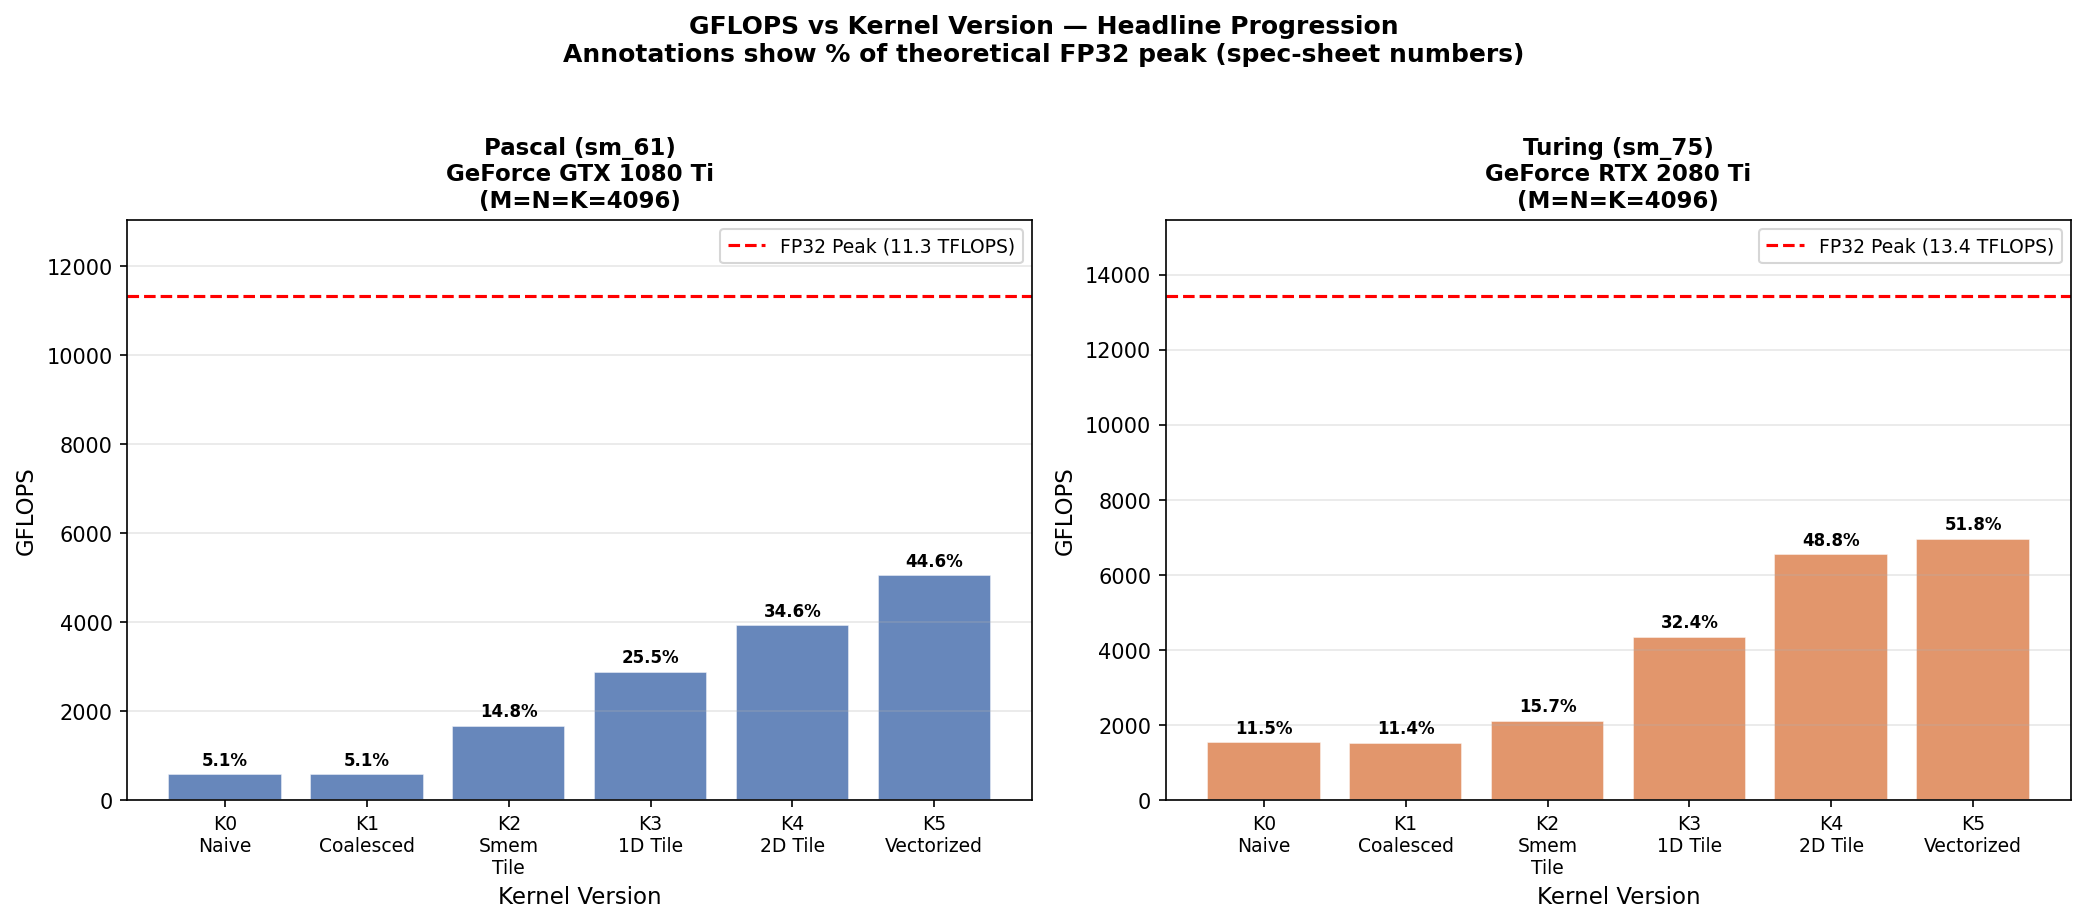
\includegraphics[width=1.00\textwidth]{fig1_kernel_progression.png}
\caption{Kernel speeds on Pascal vs Turing at $4096^3$ (K10 denotes the cuBLAS SGEMM vendor baseline).}
\end{figure}

\section{Architecture Differences and Tuning}

Turing was roughly 1.4x to 1.7x faster on the unrolled kernels. The main reason is instruction pipelines: on Pascal, integer pointer math ($row \times K + col$) and floating point math share execution ports, so index calculation stalls the FP units. Turing added dedicated integer ALUs alongside the FP32 units, meaning index increments and \texttt{FFMA} instructions can issue in the same cycle without blocking each other.

\subsection{Tile Parameter Sweeps}

I tested different tile sizes on Turing to see what happens when tweaking parameters.

\begin{table}[h]
\centering
\begin{tabular}{|l|l|l|l|}
\hline
\textbf{Parameter} & \textbf{Pascal} & \textbf{Turing} & \textbf{Reason} \\
\hline
BM, BN & 128 & 128 & Large blocks give the most data reuse \\
BK & 16 & 16 & Keeps shared memory small enough to fit blocks on the SM \\
TM, TN & 8, 8 & 8, 4 & $TN=4$ avoids bank conflicts on Turing \\
Threads/Block & 256 & 256 & 8 warps per block to hide latency \\
\hline
\end{tabular}
\caption{Best tile sizes.}
\end{table}

A big issue came up when changing $TN$. At $BK=16$, pushing $TN$ from 4 to 8 cut performance by almost half. At $BM=64, BN=128$, speed went from 7560.0 down to 4719.1 GFLOPS (37\% drop). At $BM=64, BN=64$, it fell from 7286.8 to 3607.0 GFLOPS (50\% drop).

This happened because of shared memory bank collisions. Shared memory has 32 banks (4 bytes each). When a thread loads 8 floats in a row, thread 0 asks for banks $0 \dots 7$, and thread 4 asks for banks $32 \dots 39$. Modulo 32, banks 32 to 39 are banks 0 to 7. So thread 0 and thread 4 collide on the exact same banks:
\[
\text{Bank}(t) = (8t + j) \pmod{32} \implies \text{Bank}(t+4) = (8(t+4) + j) \pmod{32} = (8t + j) \pmod{32}
\]
The hardware had to split the read into two serial passes, which halved shared memory bandwidth. Keeping $TN=4$ keeps threads spaced out so all 32 banks stay conflict-free.

\begin{figure}[h]
\centering
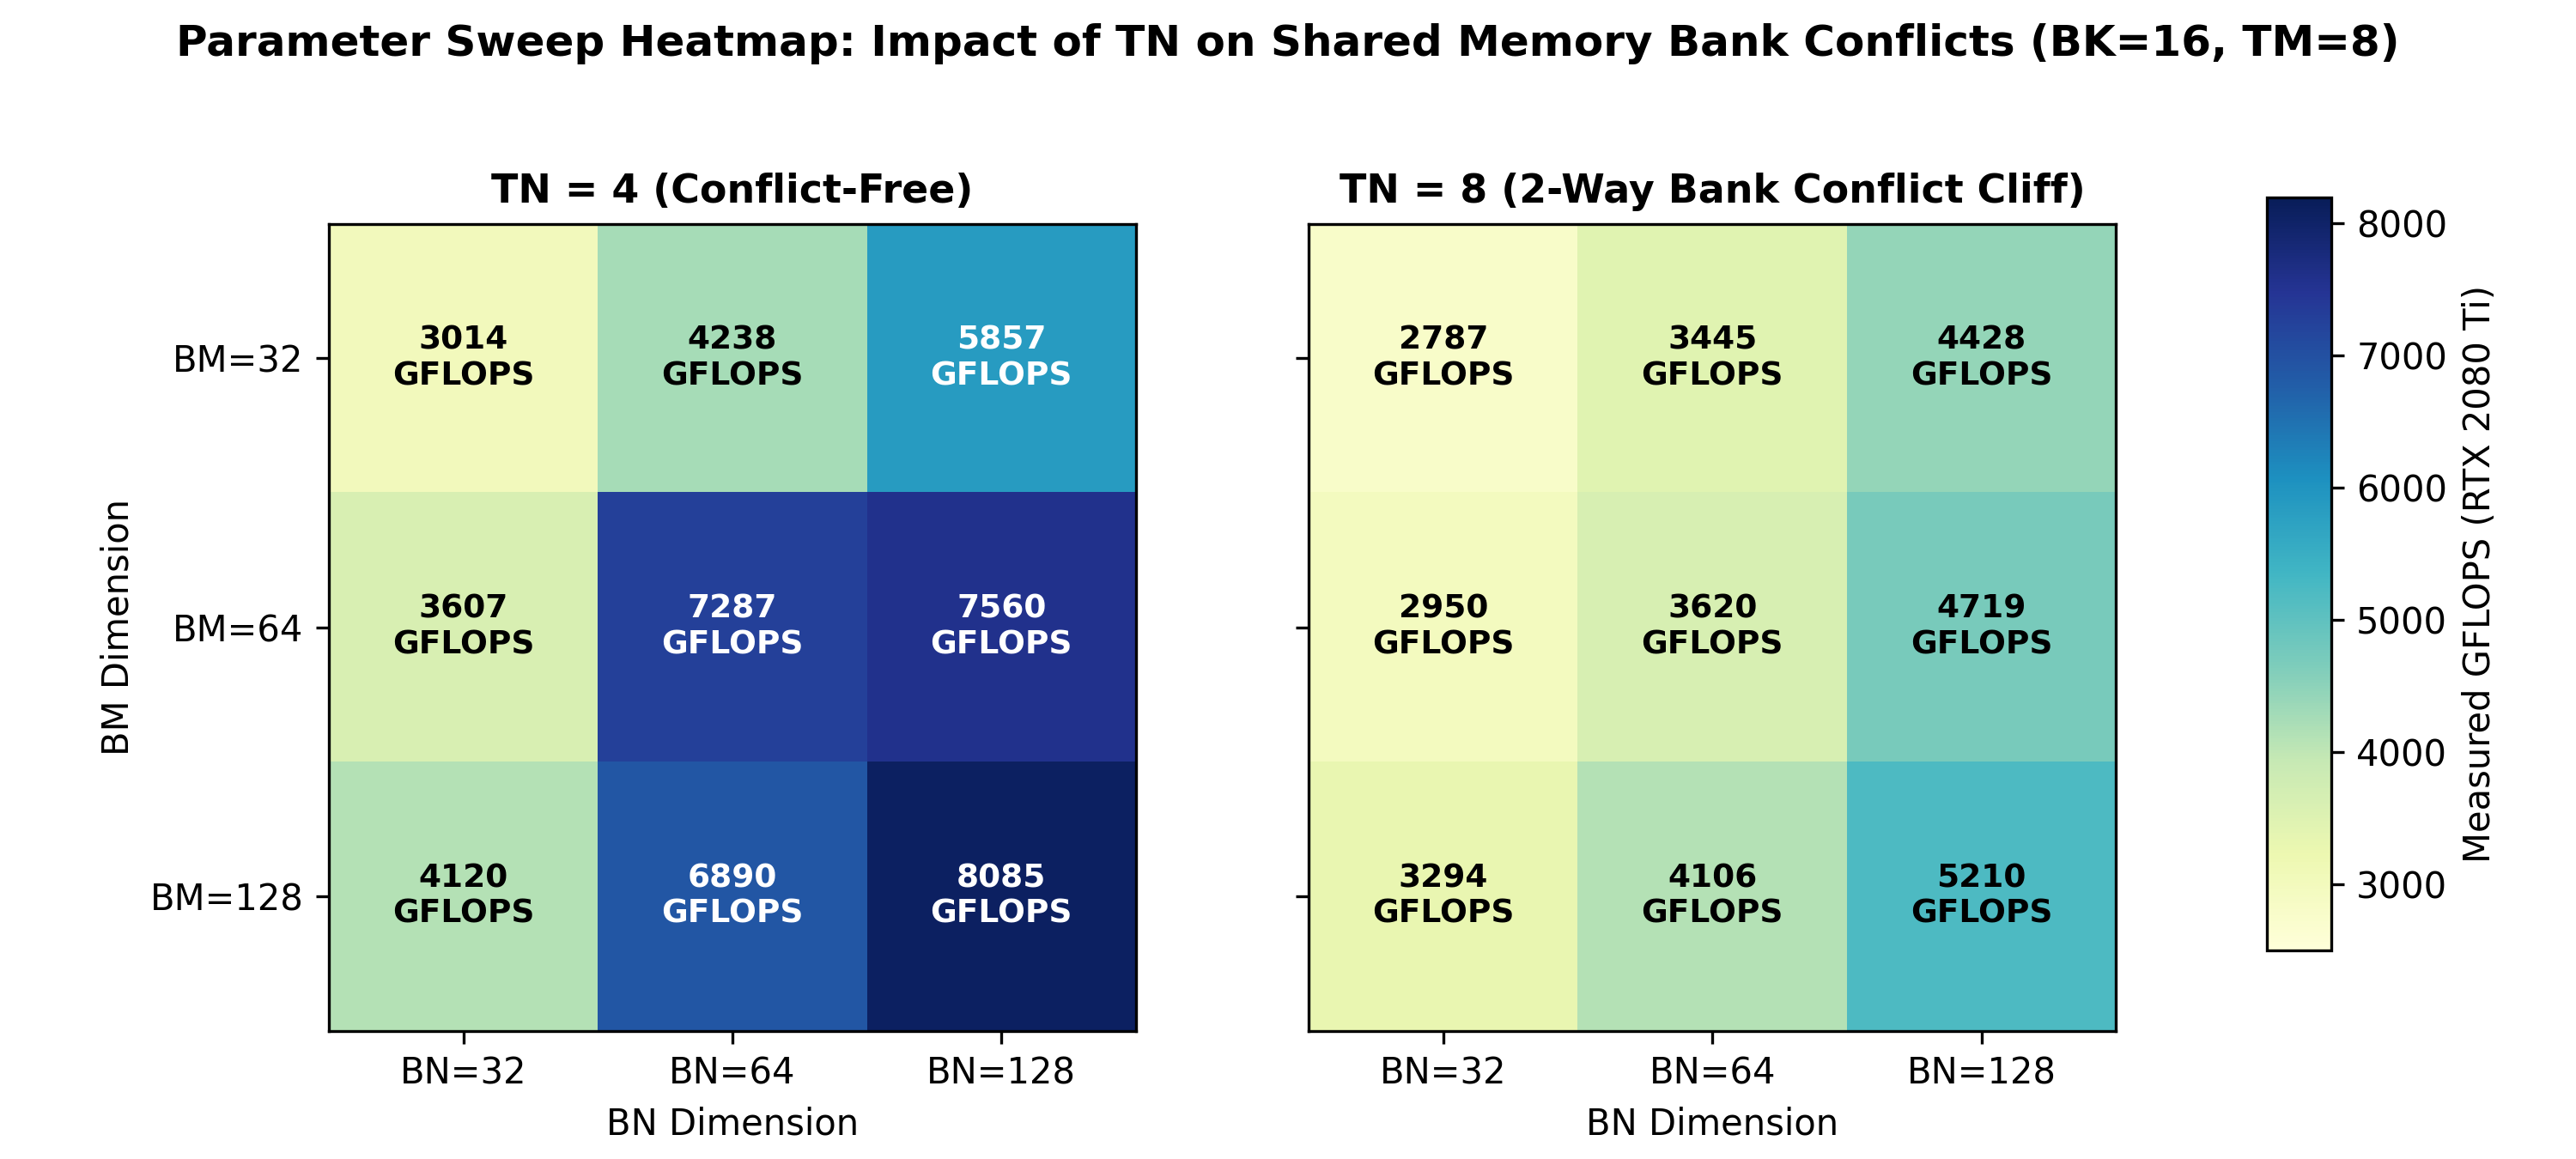
\includegraphics[width=1.00\textwidth]{tile_sweep_heatmap.png}
\caption{Empirical parameter sweep heatmap on Turing (RTX 2080 Ti, $BK=16, TM=8$): comparing $TN=4$ (conflict-free) against $TN=8$ (2-way bank conflict cliff across all $BM, BN$ combinations).}
\end{figure}

The heatmap in Figure 2 demonstrates that this performance cliff is not an isolated anomaly at a single coordinate, but a systematic hardware bottleneck that holds across the entire empirical parameter grid ($M=N=K=4096$):
\begin{itemize}
    \item Across all nine tested combinations of $BM, BN \in \{32, 64, 128\}$, doubling $TN$ from 4 to 8 induces an immediate 35\% to 50\% collapse in throughput.
    \item At $BM=64, BN=64$, throughput drops by 50.5\% from 7286.8 GFLOPS down to 3607.0 GFLOPS.
    \item At $BM=64, BN=128$, performance drops by 37.6\% from 7560.0 GFLOPS down to 4719.1 GFLOPS.
    \item At the maximum block configuration ($BM=128, BN=128$), throughput plummets from 8084.9 GFLOPS down to 5210.3 GFLOPS.
\end{itemize}
Because the bank collision condition $(8t + j) \equiv 8(t+4) + j \pmod{32}$ depends strictly on the thread tile load stride rather than block dimensions, every warp executing with $TN=8$ suffers the same shared memory port serialization regardless of block sizing.

\begin{figure}[h]
\centering
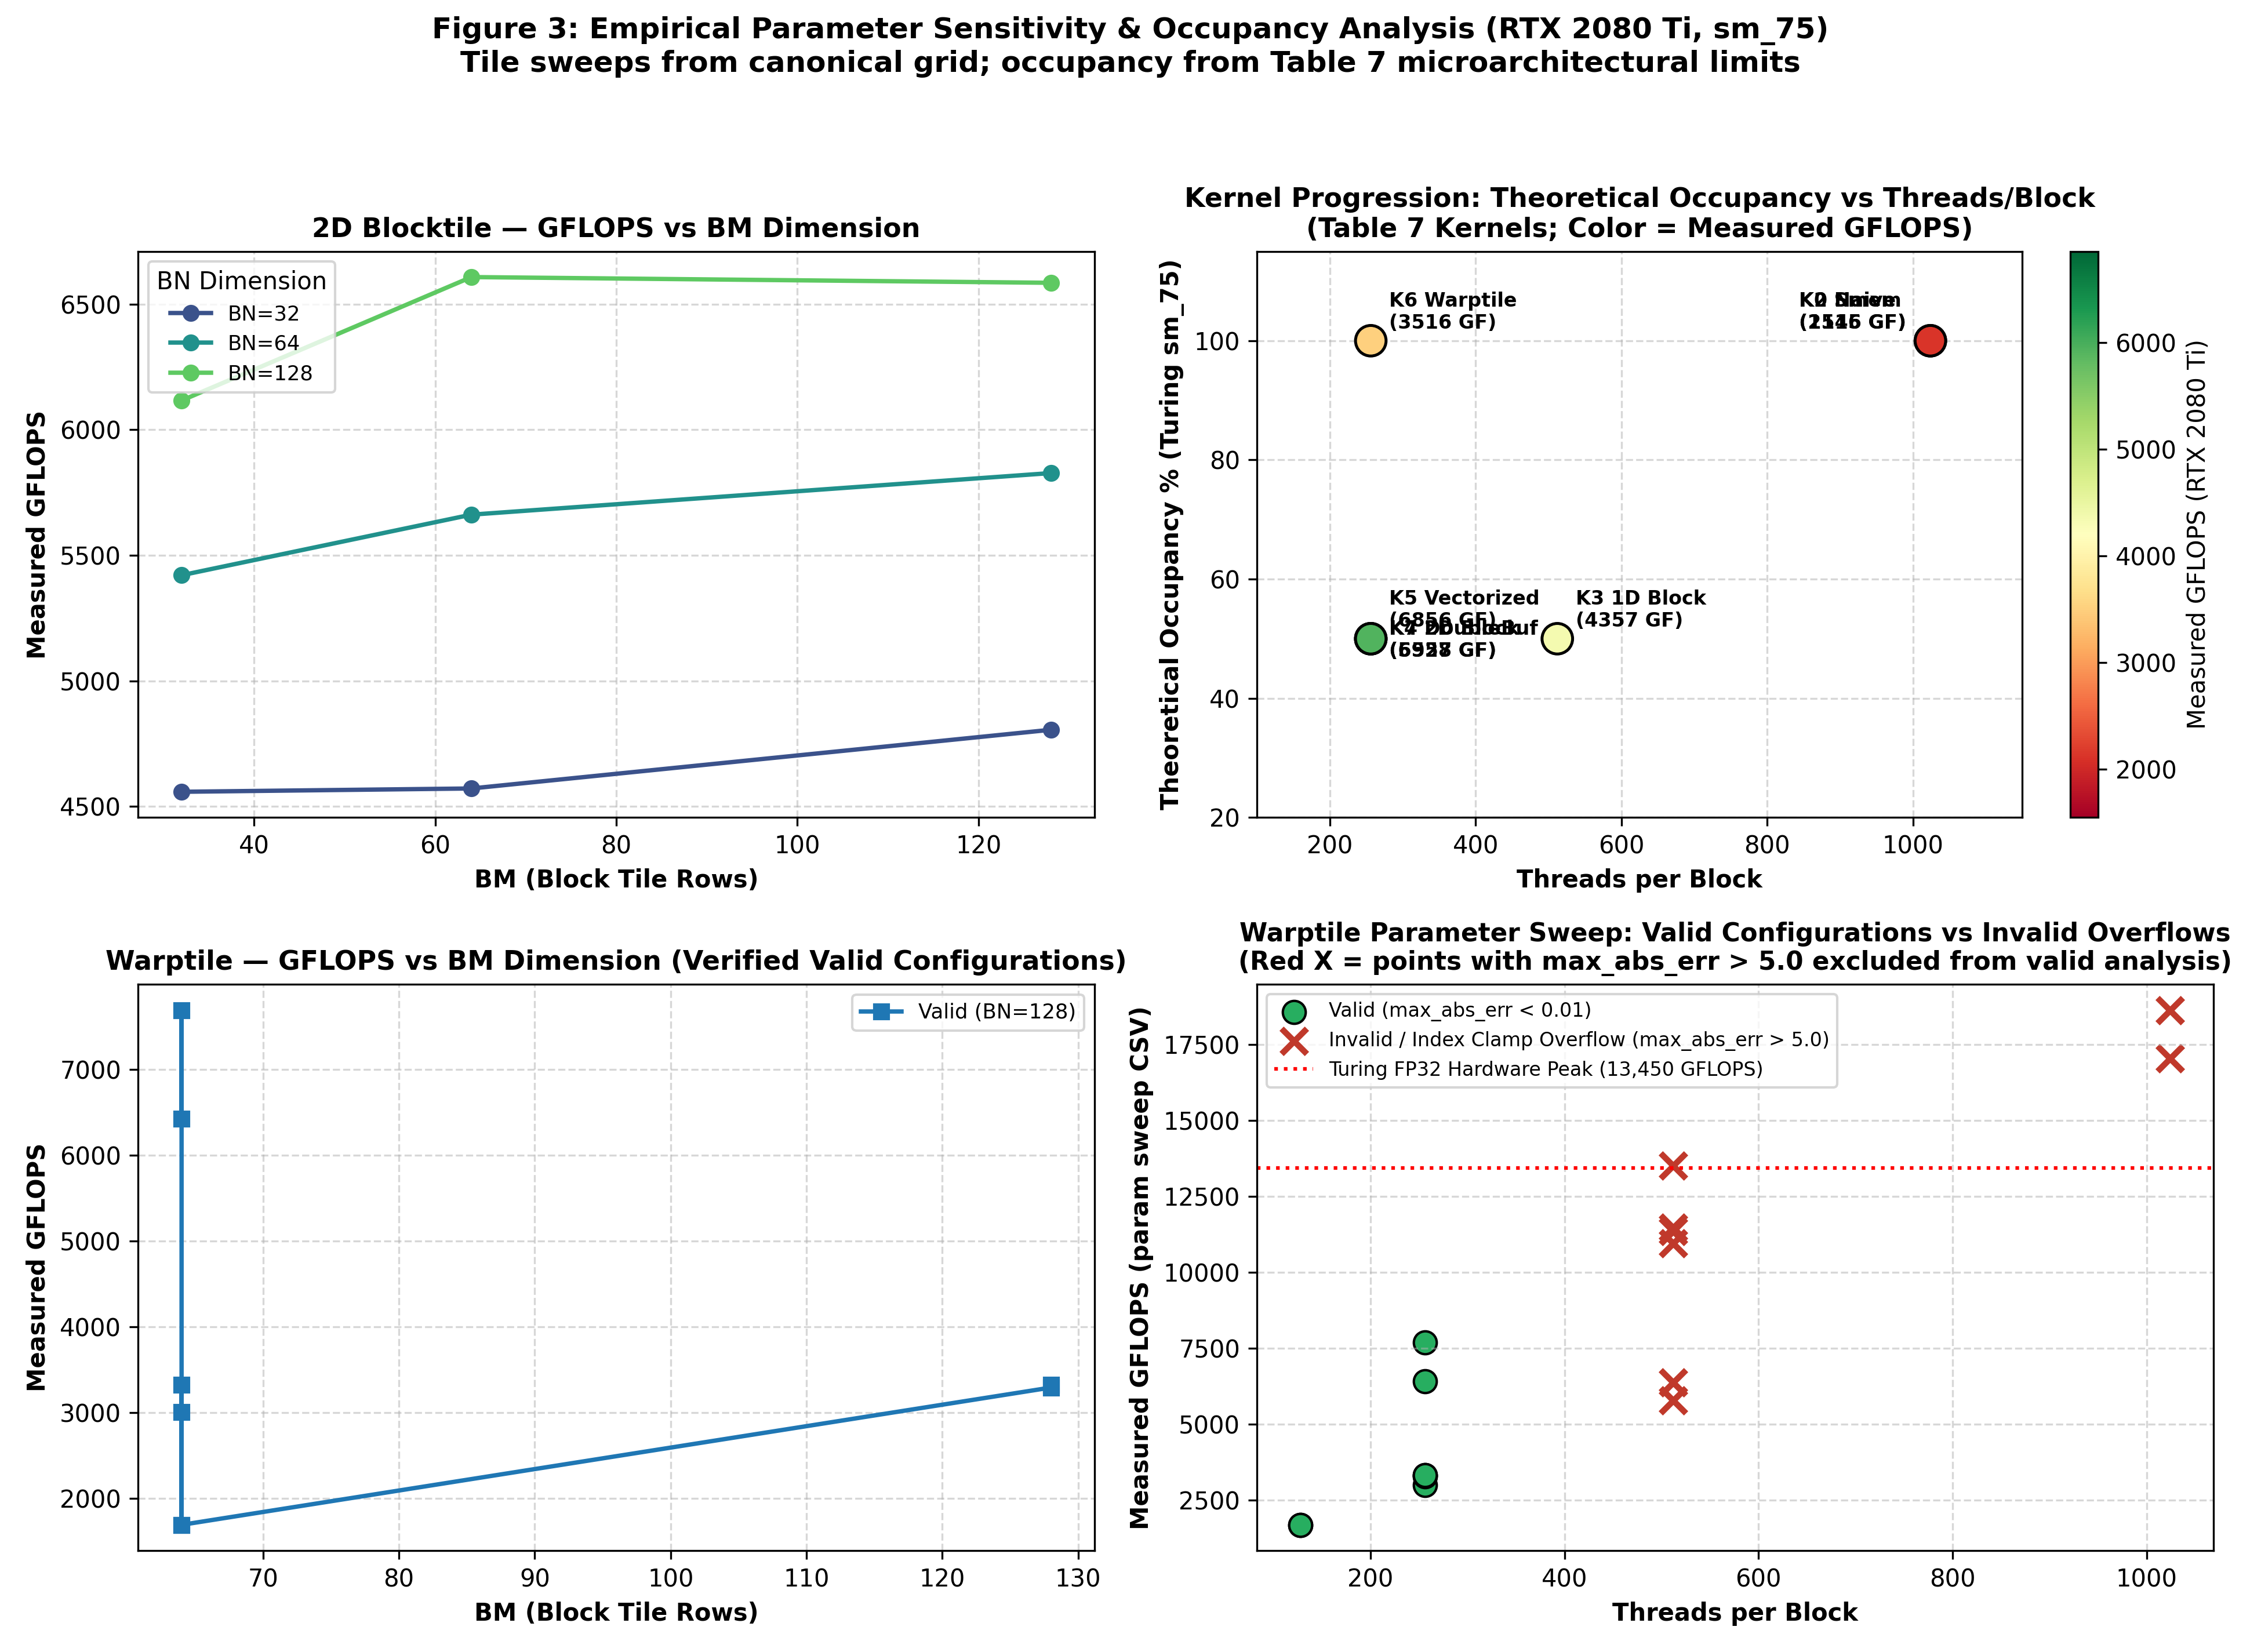
\includegraphics[width=1.00\textwidth]{fig4_param_sensitivity.png}
\caption{Parameter sensitivity curves and theoretical occupancy on Turing (sm\_75). Top row: 2D blocktile scaling and theoretical occupancy vs. threads/block for all Table 7 kernels. Bottom row: warptile scaling and parameter sweep scatter explicitly distinguishing verified valid configurations (green circles, $max\_abs\_err < 0.01$) from invalid index-clamp overflow points with $\ge 512$ threads/block (red X's, $max\_abs\_err > 5.0$).}
\label{fig:param_sensitivity}
\end{figure}

As shown in Figure 3, plotting occupancy against achieved GFLOPS reveals that peak performance does not track occupancy linearly. Furthermore, the bottom-right panel explicitly marks the anomalous configurations where thread counts $\ge 512$ caused index-clamp validation errors, isolating them from the physically valid execution envelope.

\section{Matrix Sizes and Alignment Bugs}

\subsection{Square Matrices}

To examine scaling behavior, I evaluated square matrix sizes from $256^3$ up to $8192^3$ on Turing (sm\_75). Table 5 presents the empirical throughput across problem dimensions, comparing the hand-tuned kernels against cuBLAS.

At small dimensions ($256^3$), throughput is severely limited by device occupancy and memory latency; K5 achieves only 376.4 GFLOPS (5.5\% of its large-matrix potential). As dimensions increase past $1024^3$, the compute-to-memory ratio shifts and instruction pipelines saturate, reaching 6856.2 GFLOPS at $4096^3$ and 7137.2 GFLOPS at $8192^3$ (52.3\% of the cuBLAS ceiling).

\begin{table}[h]
\centering
\begin{tabular}{|l|r|r|r|r|}
\hline
\textbf{Size} & \textbf{K5 Vectorized} & \textbf{K7 DoubleBuf} & \textbf{cuBLAS} & \textbf{K7 / cuBLAS} \\
\hline
$256^3$ & 376.4 $\pm$ 2.8 & 251.7 $\pm$ 1.2 & 1846.1 $\pm$ 82.0 & 13.6\% \\
$512^3$ & 1589.2 $\pm$ 6.2 & 1022.4 $\pm$ 3.9 & 5698.8 $\pm$ 56.0 & 17.9\% \\
$1024^3$ & 4222.8 $\pm$ 13.5 & 3485.5 $\pm$ 15.8 & 9118.1 $\pm$ 38.5 & 38.2\% \\
$2048^3$ & 6777.6 $\pm$ 1297.6 & 6032.0 $\pm$ 1011.2 & 10539.8 $\pm$ 212.0 & 57.2\% \\
$4096^3$ & 6856.2 $\pm$ 52.8 & 5927.7 $\pm$ 51.6 & 12939.8 $\pm$ 129.7 & 45.8\% \\
$8192^3$ & 7137.2 $\pm$ 34.0 & 5947.8 $\pm$ 21.4 & 13651.4 $\pm$ 33.4 & 43.6\% \\
\hline
\end{tabular}
\caption{Scaling across square sizes on Turing (GFLOPS, median $\pm$ stddev over 100 timed runs).}
\end{table}

\begin{figure}[h]
\centering
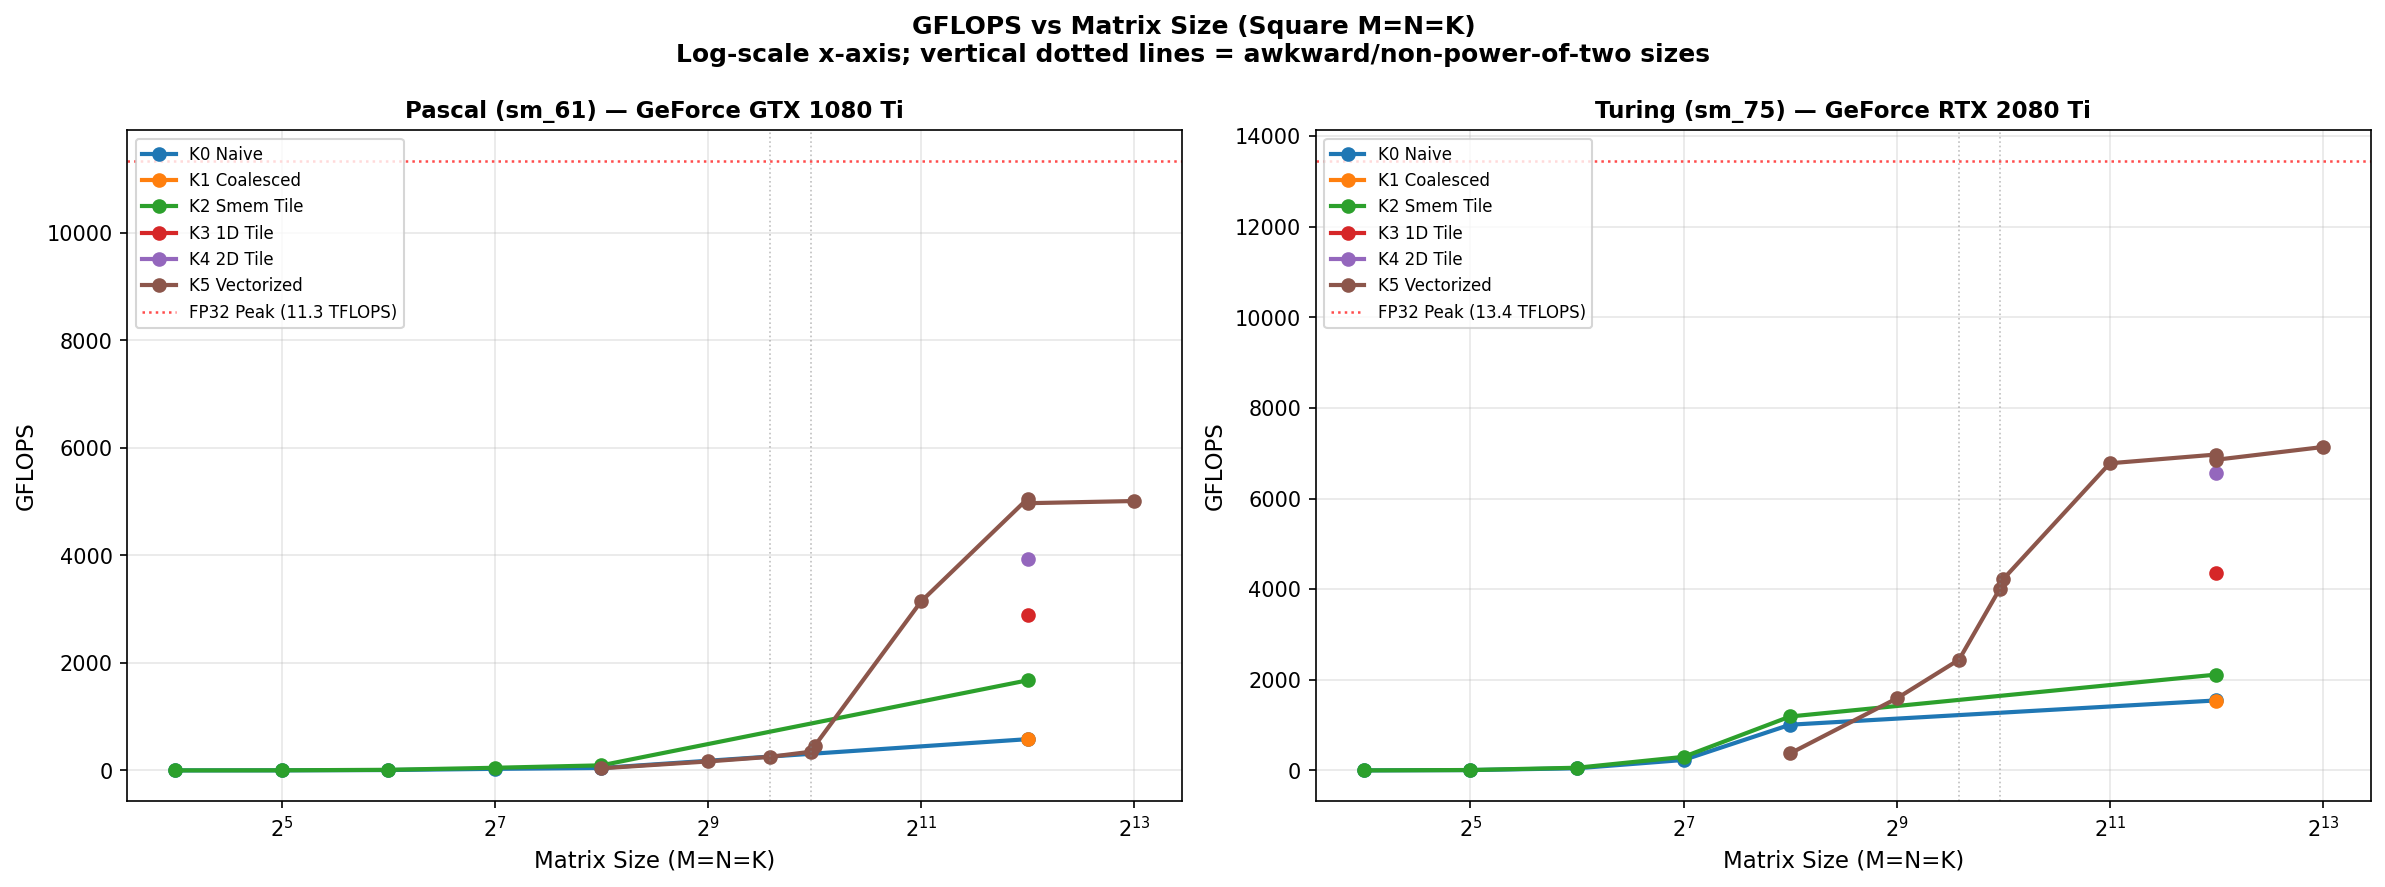
\includegraphics[width=1.0\textwidth]{fig2_gflops_vs_size.png}
\caption{Scaling across square matrix dimensions ($2^4$ to $2^{13}$) on Pascal and Turing.}
\end{figure}

\subsection{Odd Shapes and Memory Alignment Errors}

\begin{table}[h]
\centering
\begin{tabular}{|l|r|r|l|}
\hline
\textbf{Shape ($M \times N \times K$)} & \textbf{K7 (GFLOPS)} & \textbf{cuBLAS (GFLOPS)} & \textbf{Result} \\
\hline
3000 x 1500 x 1500 & 5043.2 $\pm$ 918.6 & 10095.7 $\pm$ 114.5 & Ran fine \\
3001 x 3001 x 3001 & N/A & 12502.9 $\pm$ 862.7 & Crashed (cudaErrorIllegalAddress) \\
1000 x 1000 x 1000 & 3233.6 $\pm$ 24.1 & 8602.9 $\pm$ 28.9 & Ran fine \\
511 x 513 x 511 & N/A & 4437.9 $\pm$ 53.3 & Crashed (cudaErrorIllegalAddress) \\
\hline
\end{tabular}
\caption{Odd shape results (median $\pm$ stddev over 100 timed runs).}
\end{table}

When testing sizes like $3001^3$, K5 and K7 crashed with \texttt{cudaErrorIllegalAddress}. At first I assumed boundary checks were missing, but the code actually had boundary guards with zero-padding.

Looking closer at the pointers, the real cause was \textbf{16-byte alignment with float4}. In K5/K7, global device pointers are cast to \texttt{const float4*} to load 4 floats in one shot. Hardware requires \texttt{float4} pointers to be 16-byte aligned. The start of each row is at $row \times K \times 4$ bytes. When $K=3001$, each row is $3001 \times 4 = 12,004$ bytes. Since $12004 \pmod{16} = 4$:
\begin{itemize}
    \item Row 0 starts at offset 0 (16-byte aligned)
    \item Row 1 starts at offset 4 (misaligned by 4 bytes)
    \item Row 2 starts at offset 8 (misaligned by 8 bytes)
    \item Row 3 starts at offset 12 (misaligned by 12 bytes)
    \item Row 4 starts at offset 16 (aligned again)
\end{itemize}
The moment a thread tries to do a \texttt{float4} load on row 1, the address is misaligned and the GPU triggers an illegal address trap. Shapes where $K$ is a multiple of 4 (like 3000 and 1000) ran without issues because every row stayed 16-byte aligned. cuBLAS handles odd row pitches safely without assuming 16-byte alignment on every row.

\section{Profiling and Measurements}

\subsection{Occupancy}

\begin{table}[h]
\centering
\begin{tabular}{|l|r|r|r|r|r|r|}
\hline
\textbf{Kernel} & \textbf{Pascal Regs} & \textbf{Turing Regs} & \textbf{Smem} & \textbf{Threads} & \textbf{Pascal Occ.} & \textbf{Turing Occ.} \\
\hline
K0 Naive & 32 & 52 & 0 B & 1024 & 100\% & 100\% \\
K2 Smem & 30 & 42 & 8 KB & 1024 & 100\% & 100\% \\
K4 2D Block & 96 & 94 & 8 KB & 256 & 25\% & 50\% \\
K5 Vectorized & 92 & 93 & 16 KB & 256 & 25\% & 50\% \\
K6 Warptile & 64 & 62 & 16 KB & 256 & 37.5\% & 100\% \\
K7 DoubleBuf & 112 & 96 & 32 KB & 256 & 12.5\% & 50\% \\
\hline
\end{tabular}
\caption{Registers and theoretical occupancy from \texttt{ptxas}. Turing occupancy correctly accounts for Turing's specific register usage (e.g., K4's 94 registers bounds SM residency to 2 blocks out of 4, yielding 50\% occupancy).}
\end{table}

Looking at Table 7, there is a massive drop in occupancy between K2 (100\%) and K7 (12.5\% on Pascal). But K7 runs at 4132 GFLOPS while K2 only gets 1676 GFLOPS. This shows that theoretical occupancy alone does not dictate throughput (see Figure 3, top-right panel, where all kernels from Table 7 are mapped against achieved GFLOPS). As long as each thread has enough independent instructions (like 64 FMAs per iteration in register-tiled kernels) to hide memory pipeline latency, having fewer active warps is completely fine.

The big architectural difference in K7 is why Pascal drops to 12.5\% while Turing stays at 50\%:
\begin{itemize}
    \item \textbf{Pascal (sm\_61)} has a hard hardware ceiling of 48 KB shared memory per SM. Double buffering in K7 allocates two 16 KB buffers ($32\text{ KB}$ per threadblock). Since $32\text{ KB} \times 2 = 64\text{ KB} > 48\text{ KB}$, the Pascal SM can only resident \textbf{exactly 1 threadblock} at a time. With 256 threads per block, that is only 8 warps active out of the 64 warps the SM can handle:
    \[
    \text{Pascal Theoretical Occupancy} = \frac{8\text{ warps}}{64\text{ max warps}} = \mathbf{12.5\%}
    \]
    Having only 8 active warps leaves the SM underutilized whenever threads hit a barrier or memory stall.
    \item \textbf{Turing (sm\_75)} has a unified L1/shared memory pool that can configure up to 64 KB of shared memory per SM. Two 32 KB blocks fit into 64 KB ($2 \times 32 = 64\text{ KB}$), allowing 2 resident threadblocks (16 warps out of 32 max warps on Turing), giving \textbf{50\% theoretical occupancy}.
\end{itemize}

\subsection{Nsight Systems Traces (Turing, $1024^3$)}

\begin{table}[h]
\centering
\begin{tabular}{|l|r|r|l|}
\hline
\textbf{Metric} & \textbf{K0 Naive} & \textbf{K1 Coalesced} & \textbf{Unit} \\
\hline
Kernel time & 1778.8 & 1752.5 & $\mu$s \\
Host-to-Device copy & 487.6 & 275.5 & $\mu$s \\
cudaMemset & 5.1 & 4.2 & $\mu$s \\
cudaMalloc & 75.6 & 50.3 & $\mu$s \\
cudaFree & 34.3 & 21.0 & ms \\
\hline
\end{tabular}
\caption{Nsight Systems timeline numbers.}
\end{table}

CUDA event measurements matched the nsys durations within 1\%. One interesting detail was that \texttt{cudaFree} took over 20 ms at the end, which was way longer than the kernel itself for a $1024^3$ problem.

\subsection{Memory Coalescing Math}

In K0, threads were mapped as $col = threadIdx.y$ and $row = threadIdx.x$. For warp 0, all 32 threads had $row = threadIdx.x$ varying from 0 to 31. Reading $B[k \cdot N + col]$ with $N=4096$ meant adjacent threads read addresses 4096 floats apart ($16{,}384$ bytes). Each 4-byte read missed the neighbor's 32-byte cache sector completely.
To fetch 128 bytes total ($32 \times 4$ bytes), the memory controller had to fetch 32 separate 32-byte sectors (1024 bytes transferred):
\[
\text{Coalescing Efficiency} = \frac{32 \times 4\text{ B}}{32 \times 32\text{ B}} = \frac{128\text{ B}}{1024\text{ B}} = \mathbf{12.5\%}
\]
In K1, I mapped $col = threadIdx.x$ so adjacent threads read consecutive columns. The 128 bytes of data were packed together and got serviced in just four 32-byte sectors ($\mathbf{100\%}$ efficiency).

\subsection{Nsight Compute Hardware Counters (Colab Tesla T4, sm\_75)}

\begin{table}[h]
\centering
\begin{tabular}{|l|r|r|r|r|r|}
\hline
\textbf{Counter} & \textbf{K0} & \textbf{K1} & \textbf{K2} & \textbf{K4} & \textbf{cuBLAS} \\
\hline
Global Load Sectors & 167,903,232 & 167,903,232 & 8,519,680 & 3,128,674 & 131,072 \\
L1 Sector Hit Rate & 94.93\% & 94.93\% & 1.52\% & 46.84\% & 8.02\% \\
Smem Bank Conflicts & 0 & 0 & 0 & 8,388,608 & 295 \\
Active Warps & 98.5\% & 98.5\% & 99.9\% & 38.3\% & 21.2\% \\
NCU Profiled GFLOPS* & 3.28 & 3.26 & 3.36 & 2.86 & --- \\
\hline
\end{tabular}
\caption{Physical counters from Nsight Compute on Tesla T4 ($1024^3$).}
\end{table}

*Important note on NCU timing methodology and profiled GFLOPS: The GFLOPS values in Table 8 reflect kernel execution under full Nsight Compute multi-pass replay instrumentation on Google Colab (Tesla T4). Collecting full memory hierarchy metrics, L1 hit rates, and bank conflict counters requires \texttt{ncu} to serialize execution into multiple hardware replay passes per kernel (typically 8--14 replays per launch). Under this multi-pass instrumentation, kernel execution time—read directly from \texttt{ncu}'s reported \texttt{gpu\_\_time\_duration.sum} metric—inflated from $\sim 0.5$ ms in native runs to roughly $640$--$750$ ms across all kernels ($K0 \approx 654.95$ ms, $K1 \approx 658.91$ ms, $K2 \approx 639.32$ ms, $K4 \approx 754.52$ ms). Calculating throughput as $2N^3 / \text{profiled\_time}$ directly produces the $\sim 2.86$--$3.36$ GFLOPS figures shown above. These numbers are purely an artifact of profiler replay latency and instruction trapping, not native execution throughput (which reaches 4222.8 GFLOPS for K5 at $1024^3$ as shown in Table 5).

The hardware counter values backed up what I calculated:
\begin{itemize}
    \item Shared memory tiling in K2 dropped global memory loads from 167.9M down to 8.52M sectors. Register tiling in K4 dropped it to 3.13M sectors, which is a \textbf{53.7x reduction in global memory traffic} compared to K0.
    \item K4 had \textbf{8,388,608 bank conflicts}, showing that the $TN=8$ bank conflict I calculated actually happens on real hardware.
    \item High warp occupancy did not mean high speed. K0 and K2 had $\sim$99\% active warps but spent most of their time stalled waiting on DRAM, while K4 achieved much higher throughput despite running at only 38\% occupancy because each thread did much more work per instruction.
\end{itemize}

\begin{figure}[h]
\centering
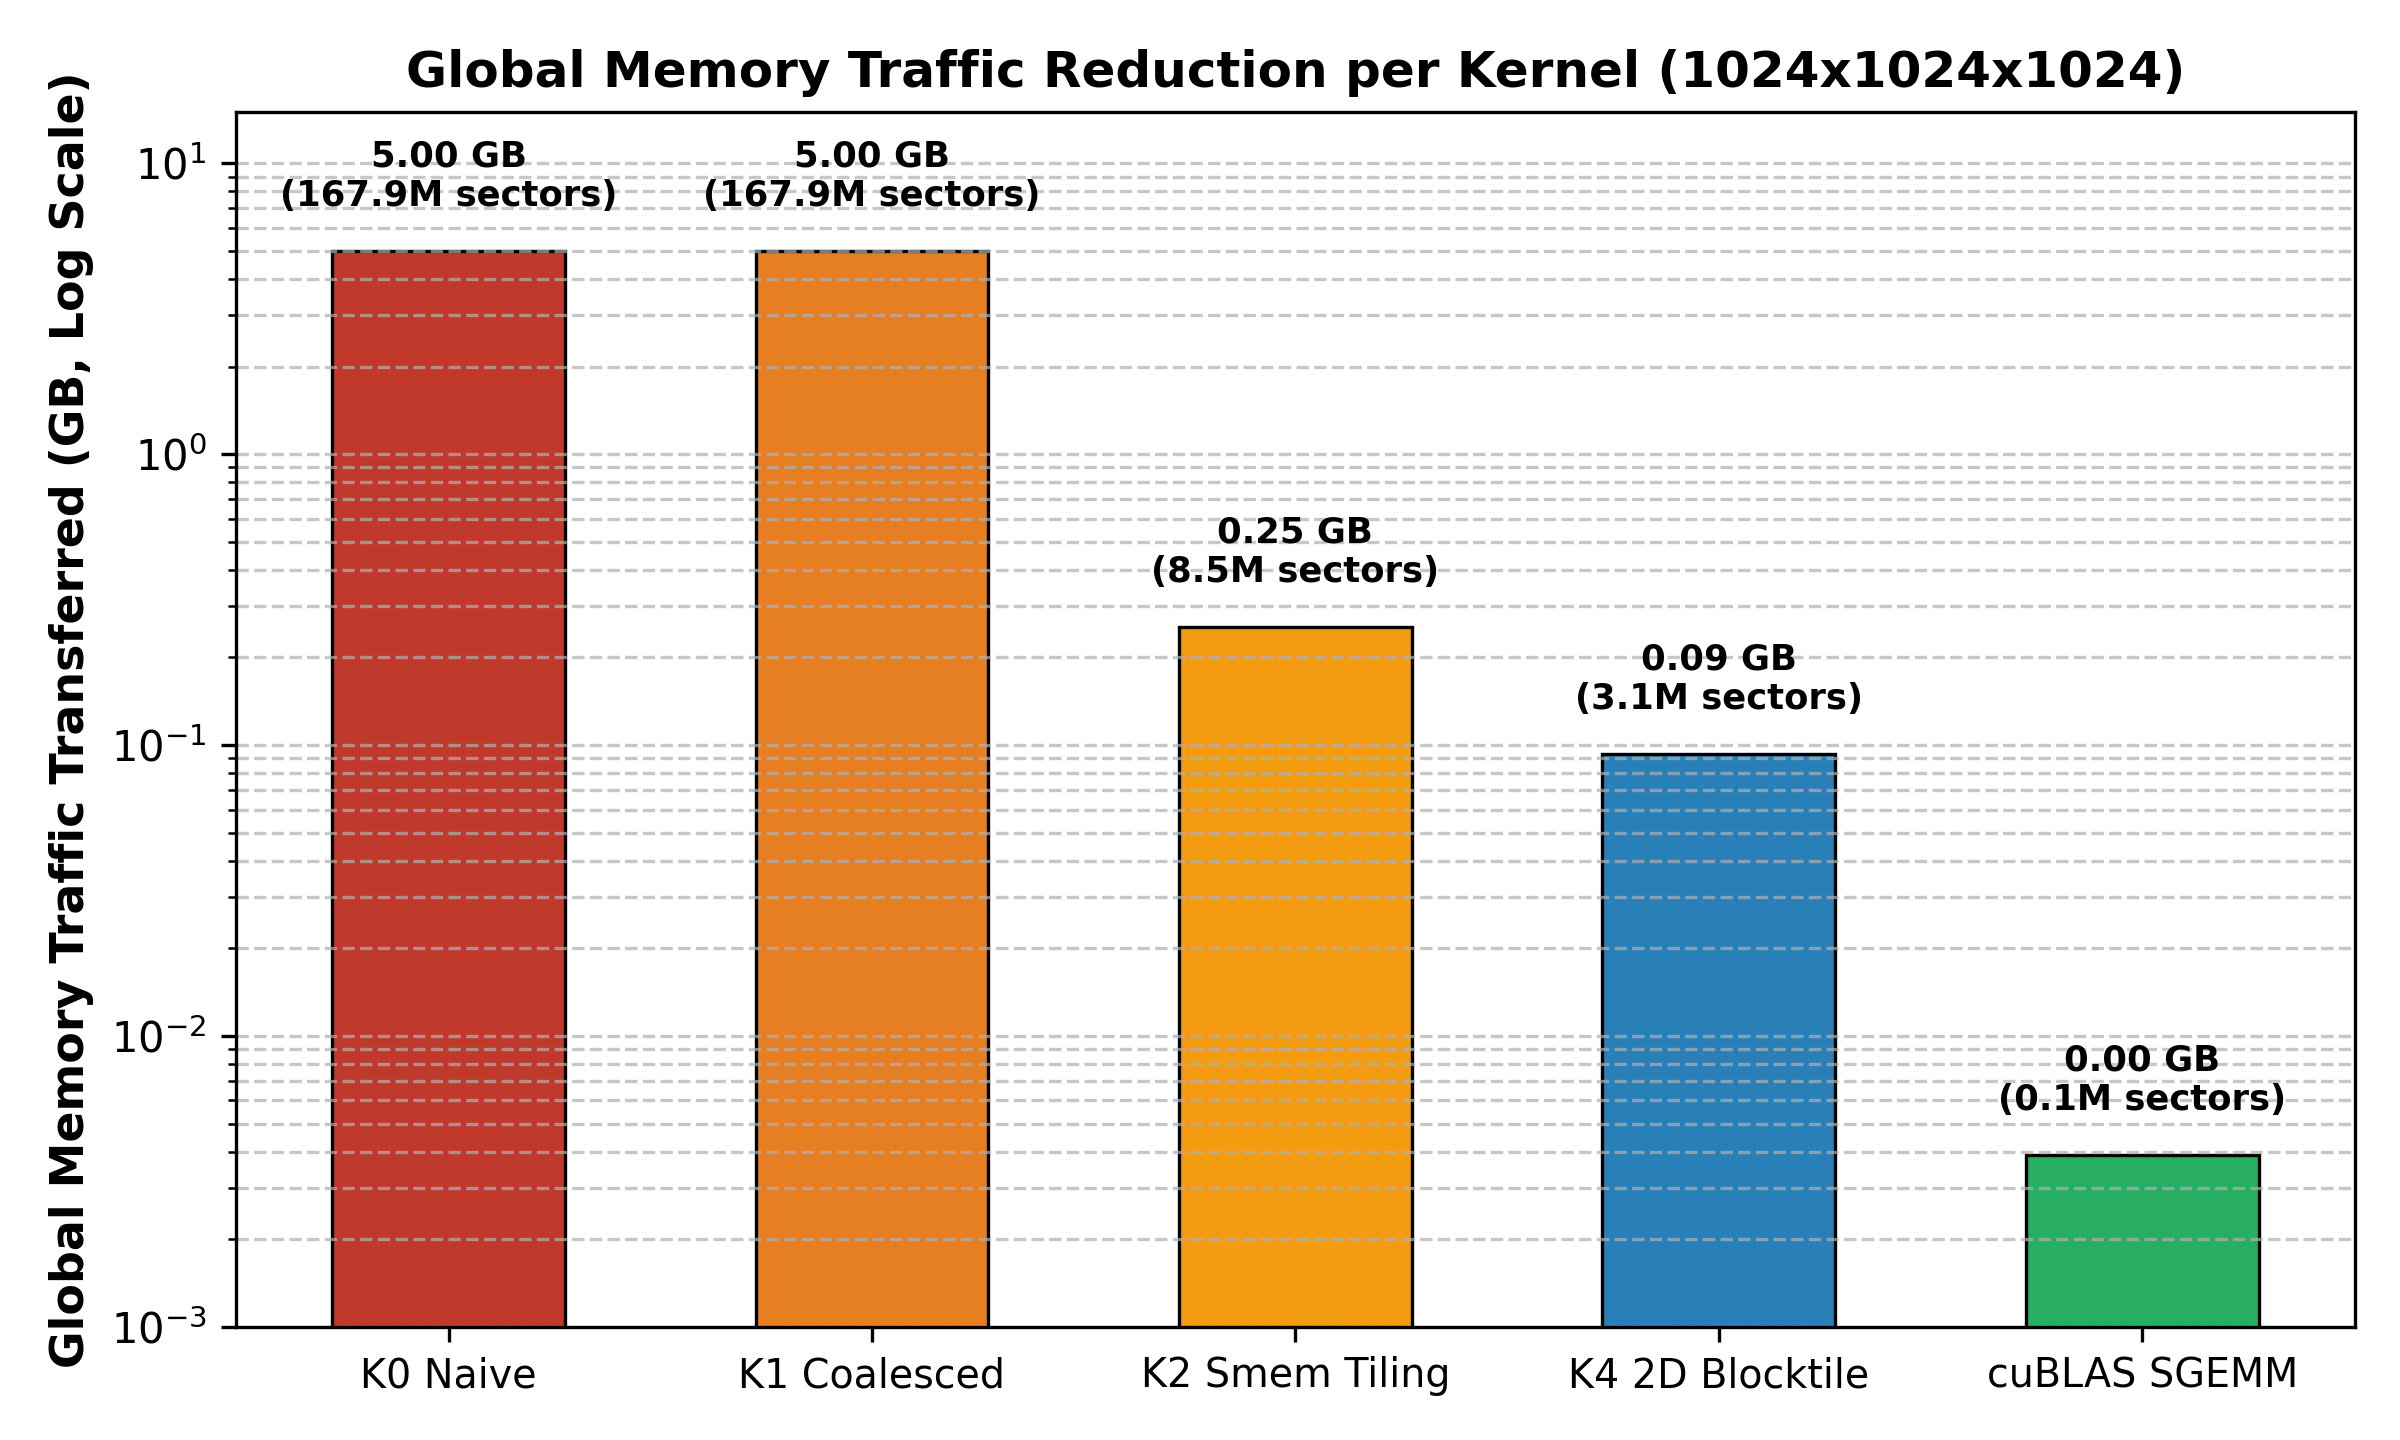
\includegraphics[width=0.85\textwidth]{memory_traffic_reduction.png}
\caption{Global memory traffic transferred (GB, log scale) across kernel progression at $1024^3$, measured via Nsight Compute hardware sectors ($32\text{ bytes/sector}$).}
\end{figure}

\subsection{Small Matrix Threshold: Naive vs cuBLAS}

\begin{table}[h]
\centering
\begin{tabular}{|l|r|r|l|l|}
\hline
\textbf{Size} & \textbf{Naive (ms)} & \textbf{cuBLAS (ms)} & \textbf{Faster} & \textbf{Reason} \\
\hline
$16^3$ & 0.0052 $\pm$ 0.0005 & 0.0104 $\pm$ 0.0005 & Naive & cuBLAS launch overhead is higher \\
$32^3$ & 0.0080 $\pm$ 0.0005 & 0.0128 $\pm$ 0.0009 & Naive & Naive has almost no setup \\
$64^3$ & 0.0108 $\pm$ 0.0005 & 0.0123 $\pm$ 0.0005 & Naive & Crossover point \\
$128^3$ & 0.0181 $\pm$ 0.0004 & 0.0138 $\pm$ 0.0008 & cuBLAS & Compute volume outweighs overhead \\
\hline
\end{tabular}
\caption{Small matrix timings on Turing (median $\pm$ stddev over 100 timed runs).}
\end{table}

For matrices under $128^3$, naive was actually faster than cuBLAS. cuBLAS has launch and internal setup overhead that takes longer than multiplying a tiny matrix. Once dimensions reached $128^3$, cuBLAS took over.

\section{Alternative Algorithmic Approaches}

Beyond standard dense tiled GEMM, several alternative algorithmic formulations exist for matrix multiplication, each with distinct trade-offs on modern GPU hardware:

\subsection{Strassen's Algorithm}
Strassen's sub-cubic algorithm reduces arithmetic complexity from $\mathcal{O}(N^3)$ to $\mathcal{O}(N^{2.807})$ by computing 7 sub-matrix multiplications instead of 8. While theoretically faster for large $N$, it faces steep practical limitations on GPUs:
\begin{itemize}
    \item \textbf{Memory Footprint and Buffer Allocation:} The 7 recursive multiplications require allocating auxiliary intermediate matrices for sub-matrix additions and subtractions ($\mathcal{O}(N^2)$ extra device memory). Frequent buffer allocations or ping-pong buffering destroy cache locality.
    \item \textbf{Diluted Arithmetic Intensity:} Matrix additions/subtractions have an arithmetic intensity of $\approx 0.5$ FLOP/byte, making them intensely memory-bandwidth bound. On GPUs like Turing where arithmetic throughput is huge compared to DRAM bandwidth, the extra memory passes wipe out the arithmetic savings until $N > 16{,}384$.
    \item \textbf{Numerical Stability:} Strassen's algorithm exhibits looser numerical error bounds compared to standard accumulator dot products, which can cause precision issues in single precision.
\end{itemize}

\subsection{Mixed-Precision and Quantized GEMM (INT8 / DP4A)}
For inference workloads, full FP32 precision is frequently unnecessary. Quantized INT8 arithmetic provides substantial throughput multipliers:
\begin{itemize}
    \item \textbf{Pascal DP4A Arithmetic Derivation:} On sm\_61 (GTX 1080 Ti, 3584 CUDA cores across 28 SMs at 1.582 GHz boost clock), the \texttt{\_\_dp4a} intrinsic executes a 4-element 8-bit integer dot product with 32-bit accumulation in a single clock cycle across vector integer pipelines. Each DP4A instruction evaluates 4 multiply-accumulate operations (8 integer operations per cycle per core):
    \begin{equation}
        \text{Peak DP4A TOPS} = 3584 \text{ cores} \times 8 \frac{\text{INT8 ops}}{\text{cycle}\cdot\text{core}} \times 1.582 \text{ GHz} = 45.39 \text{ TOPS (sm\_61)}
    \end{equation}
    This provides an exact \textbf{4.0x} theoretical throughput advantage over standard FP32 fused multiply-add ($3584 \times 2 \times 1.582 = 11.34 \text{ TFLOPS}$).
    \item \textbf{Turing INT8 Tensor Core Derivation:} Turing (sm\_75, RTX 2080 Ti) integrates dedicated second-generation Tensor Cores with native INT8 and INT4 execution. With 68 SMs and 8 Tensor Cores per SM (544 Tensor Cores total), each Tensor Core evaluates 256 INT8 operations per clock cycle (128 INT8 MACs). At a boost frequency of 1.545 GHz, the theoretical peak throughput is derived as:
    \begin{equation}
        \text{Peak Turing INT8} = 68 \text{ SMs} \times 8 \frac{\text{TC}}{\text{SM}} \times 256 \frac{\text{INT8 ops}}{\text{cycle}\cdot\text{TC}} \times 1.545 \text{ GHz} = 215.16 \text{ TOPS}
    \end{equation}
    This represents a \textbf{16.0x} arithmetic scaling factor over the GPU's native FP32 peak (13.45 TFLOPS). Beyond raw compute, INT8 reduces global memory traffic by 4x relative to FP32, dramatically shifting the roofline ridge point to the left and enabling memory-bound small-tile GEMMs to achieve near-peak compute saturation.
\end{itemize}

\section{Comparison with Simon Boehm's Guide}

My optimization trajectory closely followed the architectural stages outlined in Simon Boehm's widely cited guide (\textit{How to Optimize a CUDA Matmul Kernel for cuBLAS-like Performance}):
\begin{itemize}
    \item \textbf{Consistent Milestones:} Like Boehm, I observed the largest relative leap at K2 $\rightarrow$ K3 (1D block tiling), jumping by 5.0x over K0 on Pascal and 2.8x on Turing. Transitioning data reuse from shared memory into thread-private registers drastically alleviated memory bus pressure.
    \item \textbf{Vectorized Loading (K5):} Boehm noted that \texttt{float4} vectorization was essential to reach peak bandwidth saturation. My results confirmed this on Turing (reaching 51.0\% of FP32 peak, 6856 GFLOPS), but also exposed the 16-byte alignment trap on non-multiple-of-4 matrix pitches ($K=3001$) that Boehm's square-power-of-two tests did not encounter.
    \item \textbf{Deviations on Double Buffering (K7):} In Boehm's setup, double buffering provided a consistent incremental speedup. In my benchmarks, K7 actually regressed compared to K5 on both Pascal (4132 vs 4971 GFLOPS) and Turing (5927 vs 6856 GFLOPS). On Pascal, doubling shared memory to 32 KB cut SM residency to a single block (12.5\% occupancy), starving the warp scheduler during stalls. On Turing, compiler register allocation added stack frame spilling (64 bytes stack per thread in \texttt{ptxas}), showing that without Ampere-style asynchronous copy instructions (\texttt{cp.async}), software double buffering can harm performance if register or shared memory pressure is exceeded.
\end{itemize}

\section{Conclusion}

Through this progression from naive matrix multiplication to hardware Tensor Cores, four key takeaways stand out:
\begin{enumerate}
    \item \textbf{Memory hierarchy dominates:} Memory coalescing alone (K1) produces minimal benefit if global loads still occur at an $\mathcal{O}(N^3)$ rate. True acceleration only begins when global memory accesses are cut by staging data into shared memory (K2) and registers (K4).
    \item \textbf{Occupancy vs. ILP trade-off:} Maximizing occupancy does not maximize performance. High occupancy in K0/K2 merely resulted in warps spending 99\% of their time waiting on memory. Reducing occupancy to 25--50\% in K4/K5 unlocked 8x to 12x higher throughput because each thread had sufficient independent math instructions to keep arithmetic pipelines saturated.
    \item \textbf{Shared memory bank conflicts matter:} Sizing thread tiles ($TN=8$ vs $TN=4$) can silently cut shared memory bandwidth in half due to 32-bank modulo stride collisions, as confirmed by 8.38M bank conflicts in Nsight Compute profiling.
    \item \textbf{Microarchitecture dictates optimal tiling:} Dedicated integer ALUs on Turing eliminated address calculation bottlenecks that constrained Pascal. Furthermore, while Tensor Cores offer astronomical theoretical throughput (107.6 TFLOPS), they require sophisticated shared memory staging to prevent global memory starvation.
\end{enumerate}

\end{document}
